\documentclass{article}

\usepackage{fancyhdr}
\usepackage{extramarks}
\usepackage{amsmath,siunitx}
\usepackage{amsthm}
\usepackage{bm}
\usepackage{amssymb}
\usepackage{amsfonts}
\usepackage{multirow}
\usepackage{tikz}
\usepackage[plain]{algorithm}
\usepackage{algpseudocode}
\usepackage{changepage}
\usepackage{color}
\usepackage{hyperref}


\usetikzlibrary{automata,positioning}


%
% Basic Document Settings
%

\topmargin=-0.45in
\evensidemargin=0in
\oddsidemargin=0in
\textwidth=6.5in
\textheight=9.0in
\headsep=0.25in

\linespread{1.1}

\pagestyle{fancy}
% \lhead{\hmwkTeam}
\chead{\hmwkClass: \hmwkTitle}
\rhead{\firstxmark}
\lfoot{\lastxmark}
\cfoot{\thepage}

\renewcommand\headrulewidth{0.4pt}
\renewcommand\footrulewidth{0.4pt}

\setlength\parindent{0pt}

\newcommand{\setsep}{,    \ }

%
% Create Problem Sections
%

\newcommand{\enterProblemHeader}[1]{
    \nobreak\extramarks{}{Problem \hmwkNumber.\arabic{#1} continued on next page\ldots}\nobreak{}
    \nobreak\extramarks{Problem \hmwkNumber.\arabic{#1} (continued)}{Problem \hmwkNumber.\arabic{#1} continued on next page\ldots}\nobreak{}
}

\newcommand{\exitProblemHeader}[1]{
    \nobreak\extramarks{Problem \hmwkNumber.\arabic{#1} (continued)}{Problem \hmwkNumber.\arabic{#1} continued on next page\ldots}\nobreak{}
    \stepcounter{#1}
    \nobreak\extramarks{Problem \hmwkNumber.\arabic{#1}}{}\nobreak{}
}

\setcounter{secnumdepth}{0}
\newcounter{partCounter}
\newcounter{homeworkProblemCounter}
\setcounter{homeworkProblemCounter}{1}
\nobreak\extramarks{Problem \arabic{homeworkProblemCounter}}{}\nobreak{}

%
% Homework Problem Environment
%
% This environment takes an optional argument. When given, it will adjust the
% problem counter. This is useful for when the problems given for your
% assignment aren't sequential. See the last 3 problems of this template for an
% example.
%
\newenvironment{homeworkProblem}[2][-2]{
    \ifnum#1>0
        \setcounter{homeworkProblemCounter}{#1}
    \fi
    \section{Problem \hmwkNumber.\arabic{homeworkProblemCounter} #2}
    \setcounter{partCounter}{1}
    \enterProblemHeader{homeworkProblemCounter}
}{
    \exitProblemHeader{homeworkProblemCounter}
}

%
% Homework Details
%   - Title
%   - Due date
%   - Class
%   - Section/Time
%   - Instructor
%   - Author
%
\newcommand{\hmwkNumber}{E22}
\newcommand{\hmwkTitle}{Exam 2022}
\newcommand{\hmwkClass}{NNTI}
% \newcommand{\hmwkTeam}{Team \#25}
\newcommand{\hmwkAuthorName}{Jackie, Camilo, Kai, Dhimitrios, Hevra, Filippo}

%
% Title Page
%

\title{
    % \vspace{2in}
    \textmd{\textbf{\hmwkClass:\ \hmwkTitle}}\\
}

\author{\hmwkAuthorName}
\date \today

\renewcommand{\part}[1]{\textbf{\large Part \Alph{partCounter}}\stepcounter{partCounter}\\}

%
% Various Helper Commands
%

% Useful for algorithms
\newcommand{\alg}[1]{\textsc{\bfseries \footnotesize #1}}

% For derivatives
\newcommand{\deriv}[1]{\frac{\mathrm{d}}{\mathrm{d}x} (#1)}

% For partial derivatives
\newcommand{\pderiv}[2]{\frac{\partial}{\partial #1} (#2)}

% Integral dx
\newcommand{\dx}{\mathrm{d}x}

% Alias for the Solution section header
\newcommand{\solution}{\textbf{\large Solution}}

% Probability commands: Expectation, Variance, Covariance, Bias
\newcommand{\E}{\mathrm{E}}
\newcommand{\Var}{\mathrm{Var}}
\newcommand{\Cov}{\mathrm{Cov}}
\newcommand{\Bias}{\mathrm{Bias}}

\newenvironment{homeworkSubsection}{\begin{adjustwidth}{2.5em}{0pt}}{\end{adjustwidth}}
\newcommand{\red}[1]{\textcolor{red}{#1}}
\begin{document}

\maketitle

\begin{homeworkProblem}{Short questions}
    \subsection*{(a)}
    \begin{homeworkSubsection}
        (i) is not a good candidate because the derivative is 0 (vanishing gradient)
        (ii) is not a good candidate because the derivative is linear (exploding gradient).
        (iii) could be a candidate but the gradient also vanishes at extrema.
    \end{homeworkSubsection}
    \subsection*{(b)}
    \begin{homeworkSubsection}
        (ii) is correct because batch norm smooths the loss landscape so that the network can converge faster.
        (iii) is correct (*though it'd more precise to say "computed over each channel")
    \end{homeworkSubsection}
    \subsection*{(c)}
    \begin{homeworkSubsection}
        The problem is to calculate the batch norm, the dividend is the standard diviation which in this case is 0 (division by 0).
    \end{homeworkSubsection}
    \subsection*{(d)}
    \begin{homeworkSubsection}
        (i) Yes because the kernel depth has to match the input volumn depth

        (ii) Yes, usually one bias per kernel/filter.

        (iii) No because it only affects output dimension.

        (iv) No because it only affects output dimension.

    \end{homeworkSubsection}
    \subsection*{(e)}
    \begin{homeworkSubsection}
        Datasets that are not linearly separable are difficult for a linear classifier to correctly
        classify.
    \end{homeworkSubsection}
    \subsection*{(f)}
    \begin{homeworkSubsection}
        Because it is computationally expensive (e.g. to compute matrix inversion).
    \end{homeworkSubsection}
    \subsection*{(g)}
    \begin{homeworkSubsection}
        Efficiency (shrinking the input of the next layer) and non-linearity (introducing non-linearity to the network)
    \end{homeworkSubsection}
    \subsection*{(h)}
    \begin{homeworkSubsection}
        It is not a good idea because sigmoid function has vanishing gradient problem on large values.
    \end{homeworkSubsection}
    \subsection*{(i)}
    \begin{homeworkSubsection}
        Yes, you shuffle the data for mini batch gradient descent because you want to avoid introducing bias in the training.
        You do not need to shuffle the data for batch gradient descent because you are using the whole dataset 
        (changing rows of the input matrix does not change the output).
    \end{homeworkSubsection}
    \subsection*{(j)}
    \begin{homeworkSubsection}
        It is computational efficient.
    \end{homeworkSubsection}
\end{homeworkProblem}
\begin{homeworkProblem}{Principal Component Analysis (PCA)}
    \subsection*{(a)}
    \begin{homeworkSubsection}
        The first assumption is that the dataset are centered at 0
        i.e. the mean is substracted from each data point
        because PCA trys to project the points on the the pca hyperplane (or line)
        so that the variance of the original dataset does not change much
        and the new axes are go through the original.

        The second one is that the dataset is normalized
        because different variables (axes) have different scales.
        Their covariances are not comparable if the data are not under the same scale.
    \end{homeworkSubsection}
    \subsection*{(b)}
    \begin{homeworkSubsection}
        The objective function is given by:
        \[
            \underset{i}{\sum}||x^{(i)}-DD^\top x^{(i)}||_2
        \]
        where matrix $D \in \mathbb{R}^{m\times l}$ and vectors $x^{(i)} \in \mathbb{R}^{m}$.
        We are looking for a matrix $D$ that tranforms $x^{(i)}$ into a lower dimention($l$) space
        and minimizes the reconstruction error.
        without argmin
    \end{homeworkSubsection}
    \subsection*{(c)}
    \begin{homeworkSubsection}
        In PCA, one can think of $D^\top$ as the encoder and $D$ as the decoder with constraint $D^\top D = I$.
    \end{homeworkSubsection}
    \subsection*{(d)}
    \begin{homeworkSubsection}
        From A3.2b we know that the objective function can also be written as
        $\underset{D}{\mathrm{argmin}}||X-XDD^\top||_F^2$ and later derived as
        $\underset{D}{\mathrm{argmax}}\sum_{i=1}^{m}D_{.i}^\top X^\top XD_{.i}$
        where $D_{.i}$ is a column of $D$.
        We simplify the problem by treating $D_{.i}$ as a vector $d$ with constraint $d^\top d = 1$:
        \begin{align*}
            \underset{d}{\mathrm{argmax}}d^\top X^\top Xd
            &= \underset{d}{\mathrm{argmax}}(Xd)^2\\
            &= \underset{d}{\mathrm{argmax}}\sum_{i=1}^{n}(d^\top x^{(i)})^2\\
            &= \underset{d}{\mathrm{argmax}}\frac{1}{n}\sum_{i=1}^{n}(d^\top x^{(i)} - 0)^2
        \end{align*}
        One can observe that the formular $\frac{1}{n}\sum_{i=1}^{n}(d^\top x^{(i)} - 0)^2$ is 
        calculating the variance of the points projected onto direction $d$ (note that the mean is 0 from assumption).
    \end{homeworkSubsection}
\end{homeworkProblem}
\begin{homeworkProblem}{Machine Learning Basics}
    \subsection*{(a)}
    \begin{homeworkSubsection}
        We have the loss function $J(w) = \frac{1}{n}||Xw-y||^2_2 + \lambda w^\top w$.
        We can find the $w$ minimizes $J(W)$ by setting the gradient $\nabla_wJ(w) = 0$.
        \begin{align*}
            \nabla_wJ(w) &= 0\\
            \frac{2}{n}X^\top(Xw-y) + 2\lambda w &= 0\\
            X^\top Xw-X^\top y + n\lambda w &= 0\\
            (X^\top X + n\lambda I)w-X^\top y &= 0\\
            (X^\top X + n\lambda I)w &= X^\top y \\
            w  &=(X^\top X + n\lambda I)^{-1}X^\top y\\
        \end{align*}
    \end{homeworkSubsection}
    \subsection*{(b)}
    \begin{homeworkSubsection}
        The equation is the same as $J(w) = \frac{1}{2}||Xw-y||^2_2 + \alpha ||w||_1  + \frac{\lambda}{2}w^Tw$.
        One can observe that there is an L1 norm in the equation.
        The derivative of L1 norm cannot be expressed as a closed form because it depends on the sign of each element in vector $w$.
    \end{homeworkSubsection}
    \subsection*{(c)}
    \begin{homeworkSubsection}
        Now we have the $J(w) = \frac{1}{n}||Xw-y||^2_2 + \lambda w^\top T w$.
        Similarly we solve $\nabla_wJ(w) = 0$.
        \begin{align*}
            \frac{2}{n}X^\top(Xw-y) + \lambda (T + T^\top)w &= 0\\
            X^\top(Xw-y) + \frac{n\lambda}{2} (2T)w &= 0\\
            X^\top Xw- X^\top y + n\lambda Tw &= 0\\
            (X^\top X + n\lambda T)w &= X^\top y\\
            w &= (X^\top X + n\lambda T)^{-1}X^\top y\\
        \end{align*}
    \end{homeworkSubsection}
    \subsection*{(d)}
    \begin{homeworkSubsection}
        % We can rewrite $w^\top w$ as $w^\top (ww^\top)^{\gamma-1} w$.
        % Since $(ww^\top)^{\gamma-1}$ is symmetric matrix we can reuse the result from (c) and get
        % \[
        %     w = (X^\top X + n\lambda (ww^\top)^{\gamma-1})^{-1}X^\top y\\
        % \]
        \[
            f(w) = \lambda'(w^\top w)^\gamma = \lambda'(\underset{i}{\sum} w_i^2)^\gamma
        \]
        \[
            \frac{\partial f}{\partial w_j} = \lambda'\gamma(\underset{i}{\sum} w_i^2)^{\gamma-1}2w_j
        \]
        so
        \[
            \nabla_w f(w) = \lambda'\gamma(w^\top w)^{\gamma-1}2w
        \]
        Thus we have the gradient of the regularization term:
        \[
            \frac{\partial}{\partial w}\lambda'(w^\top w)^{\gamma} = \lambda'\gamma(w^\top w)^{\gamma-1}2w
        \]
        and the gradient of the new loss function becomes:
        \begin{align*}
            \nabla_wJ(w)    &= 0\\
            \frac{2}{n}X^\top(Xw-y) + 2\lambda'\gamma(w^\top w)^{\gamma-1}w &= 0\\
            \frac{1}{n}X^\top(Xw-y) + \lambda'\gamma(w^\top w)^{\gamma-1}w &= 0\\
            X^\top Xw-X^\top y + n\lambda'\gamma(w^\top w)^{\gamma-1}w &= 0\\
            X^\top Xw + n\lambda'\gamma(w^\top w)^{\gamma-1}w &= X^\top y\\
        \end{align*}
        which can not be solved in closed form.
    \end{homeworkSubsection}
\end{homeworkProblem}
\begin{homeworkProblem}{Feed-Forward Neural Networks}
    \subsection*{(a)}
    \begin{homeworkSubsection}
        The number of units in a shallow network grows exponentially with function complexity
        so that requires more computation and memory. 
        See \href{https://stats.stackexchange.com/questions/182734/what-is-the-difference-between-a-neural-network-and-a-deep-neural-network-and-w}{here}
        for more details.
    \end{homeworkSubsection}
    \subsection*{(b)}
    \begin{homeworkSubsection}
        A saddle point is when the first derivatives are 0 (derivatives are 0 in both x and y direction)
        but the second derivatives in x and y direction are of different signs.
        As the gradient is 0, it may stop the gradient descent process even though it is not at a minimal.
        When you go to higher dimension, the probability of finding a saddle point increases because the hessian matrix has more eigenvalues.

        \href{https://en.wikipedia.org/wiki/Second_partial_derivative_test}{Check more}
        on saddle points and Hessian.
    \end{homeworkSubsection}
    \subsection*{(c)}
    \begin{homeworkSubsection}
        Mini batch approach introduces noice to gradient estimation and can help the network escape from saddle points.

        Using a small minibatch size introduces more noise into the optimization process, which can help escape saddle points more easily.
        However, excessively small minibatches may also lead to slower convergence or instability in training due to noisy gradient estimates.

        Larger minibatches provide more accurate gradient estimates but may reduce the effectiveness of noise injection in escaping saddle points.
    \end{homeworkSubsection}
    \subsection*{(d)}
    \begin{homeworkSubsection}
        MSE (Mean square error) measures the euclidean distance between the true value and the predicted one
        which penalise the euclidean distance from the true value. It is used for regression task.
        Cross Entropy penalises the difference between the predicted probability distribution and the true probability distribution of the classes.
        It is used for classification task.
    \end{homeworkSubsection}
    \subsection*{(e)}
    \begin{homeworkSubsection}
        Quoted from Assignment 5.2:\\
        \textit{Consider a Neural Network with a single hidden layer consisting of M neurons and tanh
        activation function.For any neuron in the hidden layer, simultaneous change of sign of input
        and output weights from the neuron leads to no change in the output layer therefore producing
        an equivalent transformation.Similarly, for any pair of neurons interchange of input weights
        between the neurons and simultaneous interchange of output weights produces an equivalent
        transformation}
    \end{homeworkSubsection}
    \begin{homeworkSubsection}
    \end{homeworkSubsection}
\end{homeworkProblem}
\begin{homeworkProblem}{Regularization}
    \subsection*{(a)}
    \begin{homeworkSubsection}
        \begin{align*}
            \theta^{MAP*}   &= \underset{\theta}{\mathrm{argmax}}\;P(\theta|D)\\
                            &= \underset{\theta}{\mathrm{argmax}}\;P(\theta)P(D|\theta)\\
                            &= \underset{\theta}{\mathrm{argmax}}\;\mathrm{log}(P(\theta)P(D|\theta))\\
                            &= \underset{\theta}{\mathrm{argmax}}\;(\mathrm{log}P(\theta) + \mathrm{log}P(D|\theta))\\
                            \intertext{Omitting the expansion of the probability with normal distribution term}\\
                            &= \underset{\theta}{\mathrm{argmax}}\;-(\frac{\theta^\top\theta}{2\sigma_1^2} + \sum_{i=1}^{N}\frac{(y_i - f(x_i, \theta))^2}{2\sigma_2^2})\\
                            &= \underset{\theta}{\mathrm{argmin}}\;\frac{\sigma_2^2}{\sigma_1^2}\theta^\top\theta + \sum_{i=1}^{N}(y_i - f(x_i, \theta))^2\\
        \end{align*}
        One can observe that $\theta^\top\theta$ corresponds to the $w^\top w$ term in the L2 regularization.

        Check out this \href{http://shaofanlai.com/post/79}{article} for more details.
    \end{homeworkSubsection}
    \subsection*{(b)}
    \begin{homeworkSubsection}
        In \href{https://www.deeplearningbook.org/contents/regularization.html#pf19}{this section}
        of the Goodfellow book, the proof is covered briefly.
        The derivation below is a bit more detailed.

        We have our normal loss function $J(w)$ and $J(w^*)$ is the minimum of the loss function.
        We can approximate the loss function around $w^*$ with a second order taylor expansion:
        \begin{align*}
            \hat{J}(w)  &= J(w^*) + (w-w^*)^\top\nabla_wJ(w^*) + \frac{1}{2}(w-w^*)^\top\cdot\mathrm{Hess}(w^*)\cdot(w-w^*)\\
            \intertext{We know that $\nabla_wJ(w^*) = 0$ because we are around minimum}\\
                        &= J(w^*) + 0 + \frac{1}{2}(w-w^*)^\top\cdot\mathrm{Hess}(w^*)\cdot(w-w^*)\\
                        &= J(w^*) + \frac{1}{2}(w-w^*)^\top\cdot\mathrm{Hess}(w^*)\cdot(w-w^*)\\
        \end{align*}
        \textbf{Note that the $\hat{J}(w)$ is an approximation of our loss function around $w^*$
        which we haven't introduced any regularization term/technique yet.}

        Let us first write the weights update in a iterative manner
        so that we can observe the affect of early stopping (stop in a certain iteration before the minimum):
        \begin{align*}
            \intertext{Notation clarification: \textit{$w^{(t)}$ denotes the weights at time step $t$, $\epsilon$ is the learning rate}}\\
            w^{(t)} &= w^{(t-1)} - \epsilon\nabla_w\hat{J}(w^{(t-1)})\\
            w^{(t)} &= w^{(t-1)} - \epsilon\mathrm{Hess}(w^*)\cdot(w^{(t-1)}-w^*)\\
            \Rightarrow w^{(t)} - w^* &= w^{(t-1)} - \epsilon\mathrm{Hess}(w^*)\cdot(w^{(t-1)}-w^*) - w^* \\
                        w^{(t)} - w^* &= w^{(t-1)} - w^* - \epsilon\mathrm{Hess}(w^*)\cdot(w^{(t-1)}-w^*) \\
                        w^{(t)} - w^* &= I(w^{(t-1)} - w^*) - \epsilon\mathrm{Hess}(w^*)\cdot(w^{(t-1)}-w^*) \\
                        w^{(t)} - w^* &= (I - \epsilon\mathrm{Hess}(w^*))\cdot(w^{(t-1)}-w^*) \\
            \intertext{We can rewrite $\mathrm{Hess}(w^*)$ as $Q\Lambda Q^\top$ by eigendecomposition}\\
                        w^{(t)} - w^* &= (I - \epsilon Q\Lambda Q^\top)\cdot(w^{(t-1)}-w^*) \\
            \Rightarrow Q^\top(w^{(t)} - w^*) &= Q^\top\cdot(I - \epsilon Q\Lambda Q^\top)\cdot(w^{(t-1)}-w^*) \\
                        Q^\top(w^{(t)} - w^*) &= (Q^\top - \epsilon Q^\top Q\Lambda Q^\top)\cdot(w^{(t-1)}-w^*) \\
                        Q^\top(w^{(t)} - w^*) &= (Q^\top - \epsilon \Lambda Q^\top)\cdot(w^{(t-1)}-w^*) \\
                        Q^\top(w^{(t)} - w^*) &= (IQ^\top - \epsilon \Lambda Q^\top)\cdot(w^{(t-1)}-w^*) \\
                        Q^\top(w^{(t)} - w^*) &= (I - \epsilon\Lambda)\cdot Q^\top\cdot(w^{(t-1)}-w^*) \\
        \end{align*}
        We can show that for each time step $t$ we have $Q^\top w^{(t)} = (I - (I - \epsilon\Lambda)^t)Q^\top w^*$ by induction:
        \textbf{Base case: $t=1$}
        \begin{align*}
            Q^\top(w^{(1)} - w^*) &= (I - \epsilon\Lambda)\cdot Q^\top\cdot(w^{(0)}-w^*) \\
            Q^\top(w^{(1)} - w^*) &= (I - \epsilon\Lambda)\cdot Q^\top\cdot(0-w^*) \\
            Q^\top(w^{(1)} - w^*) &= (I - \epsilon\Lambda)\cdot Q^\top\cdot(-w^*) \\
            Q^\top w^{(1)} - Q^\top w^* &= (I - \epsilon\Lambda)\cdot Q^\top\cdot(-w^*) \\
            Q^\top w^{(1)} &= (I - \epsilon\Lambda)\cdot Q^\top\cdot(-w^*) + Q^\top w^* \\
            Q^\top w^{(1)} &= -(I - \epsilon\Lambda)\cdot Q^\top w^* + Q^\top w^* \\
            Q^\top w^{(1)} &= (I -(I - \epsilon\Lambda))\cdot Q^\top w^* \\
        \end{align*}
        \textbf{Inductive step: $t=k$}
        where we assume $Q^\top w^{(k-1)} = (I - (I - \epsilon\Lambda)^{k-1})Q^\top w^*$ we simplify it as:
        \begin{align*}
            Q^\top w^{(k-1)} = (I - (I - \epsilon\Lambda)^{k-1})Q^\top w^*\\
            \Rightarrow w^{(k-1)} =  {Q^\top}^{-1}(I - (I - \epsilon\Lambda)^{k-1})Q^\top w^*\\
            \Rightarrow w^{(k-1)} =  Q(I - (I - \epsilon\Lambda)^{k-1})Q^\top w^*\\
        \end{align*}
        replace $w^{(k-1)}$ in the equation for time step $k$:
        \begin{align*}
            Q^\top(w^{(k)} - w^*) &= (I - \epsilon\Lambda)\cdot Q^\top\cdot(w^{(k-1)}-w^*) \\
            \Rightarrow Q^\top(w^{(k)} - w^*) &= (I - \epsilon\Lambda)\cdot Q^\top\cdot(Q(I - (I - \epsilon\Lambda)^{k-1})Q^\top w^* - w^*) \\
            \Rightarrow Q^\top(w^{(k)} - w^*) &= (I - \epsilon\Lambda)\cdot Q^\top\cdot Q(I - (I - \epsilon\Lambda)^{k-1})Q^\top w^* - (I - \epsilon\Lambda)\cdot Q^\top w^*\\
            \Rightarrow Q^\top(w^{(k)} - w^*) &= (I - \epsilon\Lambda)\cdot (I - (I - \epsilon\Lambda)^{k-1})Q^\top w^* - (I - \epsilon\Lambda)\cdot Q^\top w^*\\
            \Rightarrow Q^\top(w^{(k)} - w^*) &= (I - \epsilon\Lambda)\cdot (I - (I - \epsilon\Lambda)^{k-1} - I)Q^\top w^*\\
            \Rightarrow Q^\top(w^{(k)} - w^*) &= (I - \epsilon\Lambda)\cdot (-(I - \epsilon\Lambda)^{k-1})Q^\top w^*\\
            \Rightarrow Q^\top w^{(k)} - Q^\top w^* &= (I - \epsilon\Lambda)\cdot (-(I - \epsilon\Lambda)^{k-1})Q^\top w^*\\
            \Rightarrow Q^\top w^{(k)} - Q^\top w^* &= -(I - \epsilon\Lambda)^k Q^\top w^*\\
            \Rightarrow Q^\top w^{(k)} &= Q^\top w^* -(I - \epsilon\Lambda)^k Q^\top w^*\\
            \Rightarrow Q^\top w^{(k)} &= (I -(I - \epsilon\Lambda)^k) Q^\top w^*\\
        \end{align*}
        Now we have a general formular for the weights at each time step $t$, i.e.
        \[
            Q^\top w^{(t)} = (I -(I - \epsilon\Lambda)^t) Q^\top w^*
        \]
        Let's introduce L2 regularization term into the loss function and we have the new gradient formular:
        \begin{align*}
            \nabla_w\tilde{J}(w)    &= \alpha w + \nabla_w\hat{J}(w)\\
                                    &= \alpha w + \mathrm{Hess}(w^*)(w-w^*)\\
        \end{align*}
        set it to 0 and solve for $w$:
        \begin{align*}
            \nabla_w\tilde{J}(w) &= 0\\
            \alpha w + \mathrm{Hess}(w^*)(w-w^*) &= 0\\
            \alpha w + \mathrm{Hess}(w^*)w - \mathrm{Hess}(w^*)w^* &= 0\\
            \alpha w + \mathrm{Hess}(w^*)w &= \mathrm{Hess}(w^*)w^*\\
            (\alpha I + \mathrm{Hess}(w^*))w &= \mathrm{Hess}(w^*)w^*\\
            w &= (\alpha I + \mathrm{Hess}(w^*))^{-1}\mathrm{Hess}(w^*)w^*\\
            \intertext{eigendecompose $\mathrm{Hess}(w^*)$ into $Q\Lambda Q^\top$}\\
            w &= (\alpha I + Q\Lambda Q^\top)^{-1}Q\Lambda Q^\top w^*\\
            w &= Q(\alpha I + \Lambda)^{-1}Q^\top Q\Lambda Q^\top w^*\\
            w &= Q(\alpha I + \Lambda)^{-1}\Lambda Q^\top w^*\\
            Q^\top w &= (\alpha I + \Lambda)^{-1}\Lambda Q^\top w^*\\
            \intertext{$(\alpha I + \Lambda)^{-1}\Lambda$ is a matrix with diagonal elements $\frac{\lambda_i}{\alpha + \lambda_i}$ which is the same as $1 -\frac{\alpha}{\alpha + \lambda_i} $}\\
            Q^\top w &= (I - \alpha(\alpha I + \Lambda)^{-1}) Q^\top w^*\\
        \end{align*}
        comparing this result with the iterative method we derived earlier: $Q^\top w^{(t)} = (I -(I - \epsilon\Lambda)^t) Q^\top w^*$.
        We can see that if we choose the time step $t$ and learning rate $\epsilon$ accordingly so that 
        $(I - \epsilon\Lambda)^t = \alpha(\alpha I + \Lambda)^{-1}$ the two methods are equivalent.
    \end{homeworkSubsection}
    \subsection*{(c)}
    \begin{homeworkSubsection}
        See Page 253 of \href{https://www.deeplearningbook.org/contents/regularization.html}{this chapter on regularization}.
    \end{homeworkSubsection}
\end{homeworkProblem}
\begin{homeworkProblem}{Back propagation}
    \subsection*{(a)}
    \begin{homeworkSubsection}
        \[
            y = [\frac{27}{106}, \frac{1}{106}, \frac{2}{53}, \frac{27}{53}]
        \]
    \end{homeworkSubsection}
    \subsection*{(b)}
    \begin{homeworkSubsection}
        \begin{center}
            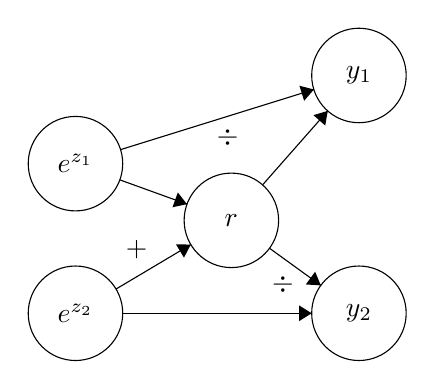
\begin{tikzpicture}[scale=0.2]
            \tikzstyle{every node}+=[inner sep=0pt]
            \draw [black] (14.9,-18) circle (3);
            \draw (14.9,-18) node {$e^{z_1}$};
            \draw [black] (14.9,-27.5) circle (3);
            \draw (14.9,-27.5) node {$e^{z_2}$};
            \draw [black] (24.8,-21.6) circle (3);
            \draw (24.8,-21.6) node {$r$};
            \draw [black] (32.9,-12.4) circle (3);
            \draw (32.9,-12.4) node {$y_1$};
            \draw [black] (32.9,-27.5) circle (3);
            \draw (32.9,-27.5) node {$y_2$};
            \draw [black] (17.48,-25.96) -- (22.22,-23.14);
            \fill [black] (22.22,-23.14) -- (21.28,-23.12) -- (21.79,-23.97);
            \draw (18.79,-24.05) node [above] {$+$};
            \draw [black] (17.72,-19.03) -- (21.98,-20.57);
            \fill [black] (21.98,-20.57) -- (21.4,-19.83) -- (21.06,-20.77);
            \draw [black] (17.76,-17.11) -- (30.04,-13.29);
            \fill [black] (30.04,-13.29) -- (29.12,-13.05) -- (29.42,-14.01);
            \draw (24.57,-15.73) node [below] {$\div$};
            \draw [black] (17.9,-27.5) -- (29.9,-27.5);
            \fill [black] (29.9,-27.5) -- (29.1,-27) -- (29.1,-28);
            \draw [black] (27.22,-23.37) -- (30.48,-25.73);
            \fill [black] (30.48,-25.73) -- (30.12,-24.86) -- (29.53,-25.67);
            \draw (28.07,-25.05) node [below] {$\div$};
            \draw [black] (26.78,-19.35) -- (30.92,-14.65);
            \fill [black] (30.92,-14.65) -- (30.01,-14.92) -- (30.76,-15.58);
            \end{tikzpicture}
            \end{center}
    \end{homeworkSubsection}
    \newpage
    \subsection*{(c)}
    \begin{homeworkSubsection}
        
        (i)\,We have these local gradients:
        \[
            \frac{\partial y}{\partial z} = \begin{pmatrix}
                \frac{\partial y_1}{\partial z_1} & \frac{\partial y_1}{\partial z_2}\\
                \frac{\partial y_2}{\partial z_1} & \frac{\partial y_2}{\partial z_2}
            \end{pmatrix} = \begin{pmatrix}
                y_1(1-y_1) & -y_1y_2\\
                -y_1y_2 & y_2(1-y_2)
            \end{pmatrix}
        \]
        (ii) The cross entropy loss looks like this: $L = -\underset{i}{\sum}y^{true}_i\mathrm{log}(y_i)$
        where $y_i$ is the prediction and $y^{true}_i$ is the true value.
        We have $\frac{\partial L}{\partial y_i} = -\frac{y^{true}_i}{y_i}$.
        Each $y_j$ is actually a function of $z_i$ so we have 
        \begin{align*}
            \frac{\partial L}{\partial z_i} &= \frac{\partial L}{\partial y_i}\cdot\frac{\partial y_i}{\partial z_i} + \underset{k\ne i}{\sum}\frac{\partial L}{\partial y_k}\cdot\frac{\partial y_k}{\partial z_i}\\
            \frac{\partial L}{\partial z_i} &= \frac{\partial L}{\partial y_i}\cdot y_i(1-y_i) + \underset{k\ne i}{\sum}\frac{\partial L}{\partial y_k}\cdot(-y_iy_k)\\
            \intertext{The result above is suffient for this question but you can simplify it further}
            &= -\frac{y^{true}_i}{y_i}\cdot y_i(1-y_i) + \underset{k\ne i}{\sum}-\frac{y^{true}_k}{y_k}\cdot(-y_iy_k)\\
            &= -y^{true}_i(1-y_i) + y_i\underset{k\ne i}{\sum}y^{true}_k\\
            &= -y^{true}_i + y^{true}_i y_i + y_i\underset{k\ne i}{\sum}y^{true}_k\\
            &= -y^{true}_i + y_i\underset{j}{\sum}y^{true}_j\\
            &= -y^{true}_i + y_i\cdot 1\\
            &= -y^{true}_i + y_i\\
        \end{align*}

        % \[
        %     \frac{\partial L}{\partial z_1} = \frac{\partial L}{\partial y_1}
        %     \cdot\frac{\partial y_1}{\partial r}
        %     \cdot\frac{\partial r}{\partial z_1}
        %     = \frac{\partial L}{\partial y_1}\cdot\frac{-e^{z_1}}{r^2}\cdot e^{z_1}
        %     = \frac{\partial L}{\partial y_1}\cdot\frac{-e^{2z_1}}{r^2}
        % \]
        % \[
        %     \frac{\partial L}{\partial z_2} = \frac{\partial L}{\partial y_2}
        %     \cdot\frac{\partial y_2}{\partial r}
        %     \cdot\frac{\partial r}{\partial z_2}
        %     = \frac{\partial L}{\partial y_2}\cdot\frac{-e^{2z_2}}{r^2}
        % \]
        % \[
        %     \frac{\partial L}{\partial r} = \frac{\partial L}{\partial y_1}
        %     \cdot\frac{\partial y_1}{\partial r} + \frac{\partial L}{\partial y_2}
        %     \cdot\frac{\partial y_2}{\partial r}
        %     = \frac{\partial L}{\partial y_1}\cdot\frac{-e^{z_1}}{r^2} +
        %     \frac{\partial L}{\partial y_2}\cdot\frac{-e^{z_2}}{r^2}
        % \]
        % (ii)\,For the general d-dimentional case, we have:
        % \[
        %     \frac{\partial L}{\partial z_i} = \frac{\partial L}{\partial y_i}
        %     \cdot\frac{\partial y_i}{\partial r}
        %     \cdot\frac{\partial r}{\partial z_i}
        %     = \frac{\partial L}{\partial y_i}\cdot\frac{-e^{2z_i}}{r^2}
        % \]
        % \[
        %     \frac{\partial L}{\partial r} = \sum_{i=1}^{d}\frac{\partial L}{\partial y_i}
        %     \cdot\frac{\partial y_i}{\partial r}
        %     = \sum_{i=1}^{d}\frac{\partial L}{\partial y_i}\cdot\frac{-e^{z_i}}{r^2}
        % \]
    \end{homeworkSubsection}
\end{homeworkProblem}
\begin{homeworkProblem}{Optimization}
    \subsection*{(a)}
    \begin{homeworkSubsection}
        i.\.RMSProp\; $\beta_1=\rho^3(1-\rho), \beta_2=\rho^2(1-\rho), \beta_3=\rho(1-\rho), \beta_4=1-\rho$

        ii.\.AdaGrad\;$\beta_i=1,\forall i$
    \end{homeworkSubsection}
    \subsection*{(b)}
    \begin{homeworkSubsection}
        We modified the term into $x_{k+1} = x_k - \alpha_k(v_k + \epsilon)$
        where $v_k = \beta v_{k-1} + (1-\beta)\nabla_f(x_k)$.
        Momentum can speed up gradient descent process. 
        It can also prevent the gradient from oscillating or overshooting.
    \end{homeworkSubsection}
\end{homeworkProblem}
\begin{homeworkProblem}{Convolutional Neural Networks}
    \subsection*{(a)}
    \begin{homeworkSubsection}
    \begin{table}[htbp]
        \centering
        \begin{tabular}{|c|c|c|c|}
            \hline
            Layer & Feature map dimensions & Number of weights & Number of biases \\
            \hline
            INPUT & $128\times128\times3$ & 0 & 0 \\
            \hline
            CONV-9-32 & $120\times120\times32$ & $9\times9\times3\times32$ & 32 \\
            \hline
            POOL-2 & $60\times60\times32$ & 0 & 0 \\
            \hline
            CONV-5-64 & $56\times56\times64$ & $5\times5\times32\times64$ & 64 \\
            \hline
            POOL-2 & $28\times28\times64$ & 0 & 0 \\
            \hline
            CONV-5-64 & $24\times24\times64$ & $5\times5\times64\times64$ & 64 \\
            \hline
            POOL-2 & $12\times12\times64$ & 0 & 0 \\
            \hline
            FC-9 & 9 & $12\times12\times64\times9$ & 1 \\
            \hline
        \end{tabular}
    \end{table}
    \end{homeworkSubsection}
    \subsection*{(b)}
    \begin{homeworkSubsection}
        \[
            y = \begin{pmatrix}
                x_1w_1 + x_2w_2\\
                x_2w_1 + x_3w_2\\
                x_3w_1 + x_4w_2\\
            \end{pmatrix}
        \]
        so we have $\nabla_wy_1= \left[x_1, x_2\right]^\top$, 
        $\nabla_wy_2= \left[x_2, x_3\right]^\top$,
        $\nabla_wy_3= \left[x_3, x_4\right]^\top$.
    \end{homeworkSubsection}
    \subsection*{(c)}
    \begin{homeworkSubsection}
        Overlapped groups allocates their gradients to the same max elements in the group
        which is explained \href{https://ai.stackexchange.com/questions/17107/how-can-we-compute-the-gradient-of-max-pooling-with-overlapping-regions}{here}.
    \end{homeworkSubsection}
    \subsection*{(d)}
    \begin{homeworkSubsection}
        In a fully connected network with one hidden layer,
        increasing in the hidden layer size will increase variance of the output.
    \end{homeworkSubsection}
\end{homeworkProblem}
\begin{homeworkProblem}{RNNs}
    See Assignment 11\\
    Question about gradient:
    \[
        \frac{\partial L}{\partial \mathbf{W}} =
        \underset{t}{\sum}\;\frac{\partial L^{(t)}}{\partial \mathbf{W}}
    \]
    List of the gradients:
    \[
        \mathbf{\delta_1^{(t)}} =
        \mathbf{\hat{y}^{(t)}} - \mathbf{y^{(t)}}
    \]
    \[
        \frac{\partial L^{(t)}}{\partial \mathbf{V}} =
        \mathbf{\delta_1^{(t)}}^\top \mathbf{h^{(t)}}^\top
    \]
    \[
        \frac{\partial L^{(t)}}{\partial \mathbf{c}} =
        \mathbf{\delta_1^{(t)}}^\top
    \]
    \[
        \mathbf{\delta_2^{(t)}} = 
        \mathbf{\delta_1^{(t)}}\cdot\mathbf{V}\cdot\mathrm{diag}(\sigma'(\mathbf{a^{(t)}}))
    \]
    \[
        \frac{\partial L^{(t)}}{\partial \mathbf{U}} =
        \mathbf{\delta_2^{(t)}}^\top\mathbf{x^{(t)}}^\top
    \]
    \[
        \frac{\partial L^{(t)}}{\partial \mathbf{W}} =
        \mathbf{\delta_2^{(t)}}^\top\mathbf{h^{(t-1)}}^\top
    \]
    \[
        \frac{\partial L^{(t)}}{\partial \mathbf{b}} =
        \mathbf{\delta_2^{(t)}}^\top
    \]
    Something is wrong with the recusive definition of $\mathbf{h}^{(t)}$

\end{homeworkProblem}


\end{document}